\documentclass[sigconf, screen, review]{acmart}
\AtBeginDocument{\providecommand\BibTeX{{Bib\TeX}}}
\setcopyright{none}\copyrightyear{2026}\acmYear{2026}\acmDOI{}
\acmConference[MICRO 2026]{The 59th IEEE/ACM International Symposium on Microarchitecture}{November 2026}{Austin, TX, USA}
\acmISBN{}\settopmatter{printfolios=true}\settopmatter{printacmref=false}
\author{Anonymous Author(s)}\affiliation{\institution{Under Review}\country{Anonymous}}
\usepackage{multirow}\usepackage{enumitem}\usepackage{tikz}
\usetikzlibrary{shapes.geometric,arrows.meta,positioning,fit,backgrounds,patterns,decorations.pathreplacing}
\usepackage{pgfplots}\pgfplotsset{compat=1.18}\usepgfplotslibrary{groupplots}\usetikzlibrary{plotmarks}
\setlength{\textfloatsep}{3pt plus 1pt minus 2pt}\setlength{\floatsep}{3pt plus 1pt minus 2pt}\setlength{\intextsep}{3pt plus 1pt minus 2pt}
\setlength{\dbltextfloatsep}{3pt plus 1pt minus 2pt}\setlength{\dblfloatsep}{3pt plus 1pt minus 2pt}\setlength{\abovecaptionskip}{1pt}\setlength{\belowcaptionskip}{0pt}
\setlength{\abovedisplayskip}{3pt plus 1pt minus 1pt}\setlength{\belowdisplayskip}{3pt plus 1pt minus 1pt}
\setlength{\parskip}{0pt plus 0.5pt}
\renewcommand{\topfraction}{0.95}\renewcommand{\bottomfraction}{0.95}\renewcommand{\textfraction}{0.05}\renewcommand{\floatpagefraction}{0.9}
\newcommand{\todo}[1]{\textcolor{red}{[TODO: #1]}}
\begin{document}
\title{A Survey of High-Level Modeling and Simulation Methods for Modern Machine Learning Workloads}\subtitle{\normalsize{MICRO 2026 Submission -- Confidential Draft -- Do NOT Distribute!!}}
\begin{abstract}
We survey 22 performance modeling tools from 53 papers (2016--2026) and evaluate five---NeuSight, ASTRA-sim, VIDUR, Timeloop, nn-Meter---across 146 GPU configurations, collective benchmarks, LLM serving, energy validation, and reproducibility testing. Three findings emerge: (1)~self-reported accuracy is unreliable---NeuSight claims 2.3\% MAPE but we measure 5.87--27.10\%, while nn-Meter produces no output due to dependency rot; (2)~the five tools are complementary but disjoint, motivating a unified pipeline; (3)~the kernel-to-model composition gap (2--9\% kernel error growing to 10--28\% model error) dominates total error, yet no tool addresses this layer.
\end{abstract}\keywords{ML workload performance prediction, DNN accelerator modeling, GPU simulation, distributed training simulation, LLM inference serving, design space exploration, survey}\maketitle
\section{Introduction}\label{sec:introduction}
Domain-specific architectures~\cite{hennessy2019golden,tpuv1_2017,tpuv4_2023} make performance prediction critical, yet no prior work examines \emph{why} certain approaches succeed or how errors propagate; prior surveys cover ML techniques for modeling~\cite{granite2022} or specific hardware. We contribute: (1)~a \textbf{28-scenario benchmark suite} where 50\% of scenarios lack tool support; (2)~\textbf{independent verification} showing claimed error rates are overstated by $2$--$4\times$; (3)~a \textbf{unified pipeline} identifying the composition gap; and (4)~a \textbf{research agenda} for composition modeling and continuous validation.
\begin{figure}[t]
\centering\resizebox{\columnwidth}{!}{%
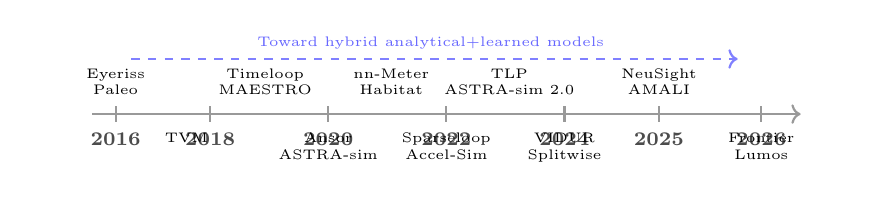
\begin{tikzpicture}[yearnode/.style={font=\scriptsize\bfseries, text=black!70}, eventnode/.style={font=\tiny, text width=2cm, align=center}]
\draw[thick, ->, black!40] (0,0) -- (9,0); \foreach \x/\year in {0.3/2016, 1.5/2018, 3/2020, 4.5/2022, 6/2024, 7.2/2025, 8.5/2026} { \draw[thick, black!40] (\x,-0.1) -- (\x,0.1); \node[yearnode, below] at (\x,-0.12) {\year}; }
\node[eventnode, above] at (0.3,0.12) {Eyeriss\\Paleo}; \node[eventnode, below] at (1.2,-0.12) {TVM}; \node[eventnode, above] at (2.2,0.12) {Timeloop\\MAESTRO}; \node[eventnode, below] at (3,-0.12) {Ansor\\ASTRA-sim}; \node[eventnode, above] at (3.8,0.12) {nn-Meter\\Habitat}; \node[eventnode, below] at (4.5,-0.12) {Sparseloop\\Accel-Sim}; \node[eventnode, above] at (5.3,0.12) {TLP\\ASTRA-sim 2.0}; \node[eventnode, below] at (6,-0.12) {VIDUR\\Splitwise}; \node[eventnode, above] at (7.2,0.12) {NeuSight\\AMALI}; \node[eventnode, below] at (8.5,-0.12) {Frontier\\Lumos};
\draw[thick, ->, blue!50, dashed] (0.5,0.7) -- (8.2,0.7); \node[font=\tiny, text=blue!60, above] at (4.3,0.7) {Toward hybrid analytical+learned models};
\end{tikzpicture}}\caption{Evolution of performance modeling tools (2016--2026).}\label{fig:timeline}\end{figure}
\section{Survey Methodology}\label{sec:methodology}
From 287 candidates on ACM DL, IEEE Xplore, Semantic Scholar, and arXiv, 53 papers (2016--2026) plus 12 foundational works were classified by methodology, platform, and abstraction level~\cite{rakhshanfar2021survey}, excluding proprietary tools, infrastructure~\cite{binkert2011gem5,sst2012}, compilers~\cite{halide2013,mlir2020,triton2019}, and schedulers~\cite{pollux2021,sia2023}.
\section{Background}\label{sec:background}
ML workloads expressed in frameworks such as PyTorch~\cite{pytorch2019} and TensorFlow~\cite{tensorflow2016} are computation graphs where performance depends on dataflow/tiling, KV cache~\cite{vllm2023}, and compute--memory--network balance; LLM inference splits into compute-bound prefill and memory-bound decode~\cite{splitwise2024,sarathi2024,orca2022}, forcing serving systems to disaggregate or chunk requests~\cite{distserve2024}; at-scale challenges such as expert parallelism~\cite{llama3scaling2025} further complicate prediction.
Five modeling types span accuracy--speed trade-offs: \textbf{analytical}~\cite{williams2009roofline,rooflinellm2024} ($\mu$s), \textbf{cycle-accurate}~\cite{gpgpusim2009,accelsim2020,dissectinggpu2025} with memory models such as DRAMSim3~\cite{dramsim3_2020} and Ramulator~\cite{ramulator2015,ramulator2_2023} ($10^3$--$10^4\times$ slowdown), \textbf{trace-driven}~\cite{astrasim2023,vidur2024} (min.), \textbf{ML-augmented}~\cite{nnmeter2021} (ms), and \textbf{hybrid}~\cite{neusight2025,habitat2021}.
\section{Taxonomy}\label{sec:taxonomy}
We organize the literature by \emph{methodology type}, \emph{target platform}, and \emph{abstraction level} (Table~\ref{tab:taxonomy-matrix}).\begin{table*}[t]
\centering\caption{Methodology taxonomy: coverage matrix and trade-off profile. \textbf{0} = research gap.}\label{tab:taxonomy-matrix}\footnotesize\begin{tabular}{l|ccccc|cccc}\toprule
 & \textbf{DNN} & & \textbf{Distrib.} & \textbf{Edge/} & & \textbf{Eval.} & \textbf{Data} & & \textbf{Failure} \\
\textbf{Methodology} & \textbf{Accel.} & \textbf{GPU} & \textbf{Systems} & \textbf{Mobile} & \textbf{CPU} & \textbf{Speed} & \textbf{Req.} & \textbf{Interp.} & \textbf{Mode} \\ \midrule
Analytical & 3 & 3 & 2 & \textbf{0} & \textbf{0} & $\mu$s & None & High & Dynamic effects \\
Cycle-Accurate & 1 & 2 & \textbf{0} & \textbf{0} & 1 & Hours & Binary & High & Scale \\
Trace-Driven & \textbf{0} & \textbf{0} & 7 & \textbf{0} & \textbf{0} & Min. & Traces & Med. & Trace fidelity \\
ML-Augmented & \textbf{0} & 3 & \textbf{0} & 3 & 1 & ms & Profiling & Low & Distrib.\ shift \\
Hybrid & 1 & 2 & \textbf{0} & \textbf{0} & 1 & ms & Mixed & Med. & Training domain \\ \bottomrule
\end{tabular}\end{table*}
Three gaps emerge (Figure~\ref{fig:tool-architecture}): trace-driven methods are exclusive to distributed systems, edge devices lack hybrid tools, and no ML-augmented tool targets distributed settings.%
\begin{figure}[t]
\centering\resizebox{\columnwidth}{!}{%
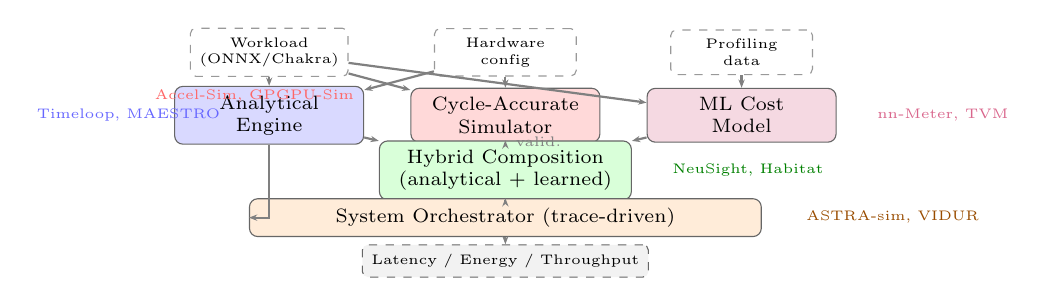
\begin{tikzpicture}[comp/.style={draw=black!60, rounded corners=3pt, minimum width=2.4cm, minimum height=0.45cm, align=center, font=\scriptsize}, input/.style={draw=black!40, dashed, rounded corners=2pt, minimum width=1.8cm, minimum height=0.35cm, align=center, font=\tiny}, arr/.style={-{Stealth[length=3pt]}, thick, black!50}, lbl/.style={font=\tiny, text=black!50}]
\node[input] (wl) at (0,1.9) {Workload\\(ONNX/Chakra)}; \node[input] (hw) at (3,1.9) {Hardware\\config}; \node[input] (prof) at (6,1.9) {Profiling\\data}; \node[comp, fill=blue!15] (analytical) at (0,1.1) {Analytical\\Engine}; \node[comp, fill=red!15] (simulator) at (3,1.1) {Cycle-Accurate\\Simulator}; \node[comp, fill=purple!15] (mlmodel) at (6,1.1) {ML Cost\\Model};
\node[comp, fill=green!15, minimum width=3.2cm] (hybrid) at (3,0.4) {Hybrid Composition\\(analytical + learned)}; \node[comp, fill=orange!15, minimum width=6.5cm] (system) at (3,-0.2) {System Orchestrator (trace-driven)}; \node[input, draw=black!60, fill=gray!10] (output) at (3,-0.75) {Latency / Energy / Throughput};
\draw[arr] (wl) -- (analytical); \draw[arr] (hw) -- (analytical); \draw[arr] (hw) -- (simulator); \draw[arr] (wl) -- (simulator); \draw[arr] (prof) -- (mlmodel); \draw[arr] (wl) -- (mlmodel); \draw[arr] (analytical) -- (hybrid); \draw[arr] (mlmodel) -- (hybrid); \draw[arr, dashed, gray] (simulator) -- node[lbl, right] {valid.} (hybrid); \draw[arr] (hybrid) -- (system); \draw[arr] (analytical) |- (system); \draw[arr] (system) -- (output);
\node[font=\tiny, text=blue!60, anchor=east] at (-0.5,1.1) {Timeloop, MAESTRO}; \node[font=\tiny, text=red!60, anchor=east] at (1.2,1.35) {Accel-Sim, GPGPU-Sim}; \node[font=\tiny, text=purple!60, anchor=west] at (7.6,1.1) {nn-Meter, TVM}; \node[font=\tiny, text=green!50!black, anchor=west] at (5,0.4) {NeuSight, Habitat}; \node[font=\tiny, text=orange!60!black, anchor=west] at (6.7,-0.2) {ASTRA-sim, VIDUR};
\end{tikzpicture}}\caption{Unified architecture showing how tool methodologies compose.}\label{fig:tool-architecture}\end{figure}
\textbf{Methodology--platform pairings.}\label{subsec:by-methodology} Platform constrains methodology: accelerators use analytical models~\cite{timeloop2019,maestro2019}; GPUs span all five types; distributed systems need trace-driven simulation~\cite{astrasim2023,vidur2024}; edge relies on ML-augmented~\cite{nnmeter2021,litepred2024}; CPUs remain the least studied platform~\cite{concorde2025}. Errors propagate (Figure~\ref{fig:abstraction-levels}): kernel 2--3\%, model 5--12\%, system 5--15\%.
\begin{figure}[t]
\centering\resizebox{\columnwidth}{!}{%
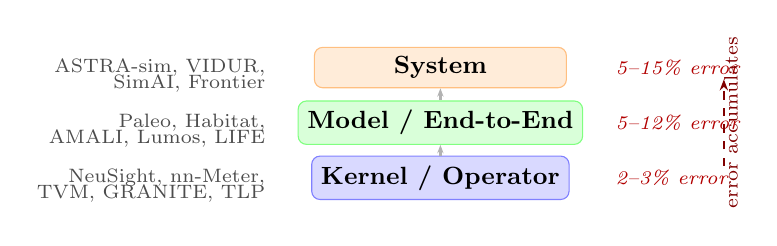
\begin{tikzpicture}[level/.style={draw, rounded corners=3pt, minimum width=3.2cm, minimum height=0.5cm, align=center, font=\small\bfseries}, tool/.style={font=\scriptsize, text=black!70}, err/.style={font=\scriptsize\itshape, text=red!70!black}, arrow/.style={-{Stealth[length=3pt]}, thick, gray!60}, compos/.style={-{Stealth[length=4pt]}, thick, red!50!black, dashed}]
\node[level, fill=blue!15, draw=blue!50] (kernel) at (0,0) {Kernel / Operator}; \node[level, fill=green!15, draw=green!50] (model) at (0,0.7) {Model / End-to-End}; \node[level, fill=orange!15, draw=orange!50] (system) at (0,1.4) {System}; \draw[arrow] (kernel) -- (model); \draw[arrow] (model) -- (system);
\node[tool, anchor=east] at (-2.1,0) {NeuSight, nn-Meter,}; \node[tool, anchor=east] at (-2.1,-0.2) {TVM, GRANITE, TLP}; \node[tool, anchor=east] at (-2.1,0.7) {Paleo, Habitat,}; \node[tool, anchor=east] at (-2.1,0.5) {AMALI, Lumos, LIFE}; \node[tool, anchor=east] at (-2.1,1.4) {ASTRA-sim, VIDUR,}; \node[tool, anchor=east] at (-2.1,1.2) {SimAI, Frontier}; \node[err, anchor=west] at (2.1,0) {2--3\% error}; \node[err, anchor=west] at (2.1,0.7) {5--12\% error}; \node[err, anchor=west] at (2.1,1.4) {5--15\% error};
\draw[compos] (3.6,0.15) -- (3.6,1.25); \node[font=\scriptsize, text=red!50!black, rotate=90, anchor=south] at (3.9,0.7) {error accumulates};
\end{tikzpicture}}\caption{Abstraction level hierarchy with error accumulation.}\label{fig:abstraction-levels}\end{figure}
\textbf{Workload coverage.}\label{subsec:workload-coverage} Of 14 tools, 9 validate only on CNNs; post-2023 tools target transformers/LLMs but \textbf{none validates on diffusion or dynamic inference} such as speculative decoding~\cite{medusa2024,dynamicreasoning2026}; only Frontier~\cite{frontier2025} covers MoE, whose expert-parallel routing introduces load-dependent latency that static models cannot capture.
\section{Survey of Approaches}\label{sec:survey}
We survey tools by target platform (Table~\ref{tab:survey-summary}).\begin{table*}[t]
\centering\caption{Surveyed tools by target platform. A=Analytical, S=Simulation, T=Trace-driven, M=ML-augmented, H=Hybrid. $^*$Surrogate-vs-simulator fidelity. $^\dagger$Unverifiable. $^\ddagger$No hardware baseline.}\label{tab:survey-summary}
\footnotesize\begin{tabular}{lllllll}\toprule
\textbf{Tool} & \textbf{Platform} & \textbf{Method} & \textbf{Target} & \textbf{Accuracy} & \textbf{Speed} & \textbf{Key Capability} \\ \midrule
\multicolumn{7}{l}{\textit{DNN Accelerator Modeling}} \\
Timeloop~\cite{timeloop2019} & NPU & A & Latency/Energy & 5--10\% & $\mu$s & Loop-nest DSE \\
MAESTRO~\cite{maestro2019} & NPU & A & Latency/Energy & 5--15\% & $\mu$s & Data-centric directives \\
Sparseloop~\cite{sparseloop2022} & NPU & A & Sparse tensors & 5--10\% & $\mu$s & Compression modeling \\
PyTorchSim~\cite{pytorchsim2025} & NPU & S & Cycle-accurate & N/A$^\ddagger$ & Hours & PyTorch 2 integration \\
ArchGym~\cite{archgym2023} & Multi & H & Multi-objective & 0.61\%$^*$ & ms & ML-aided DSE \\ \midrule
\multicolumn{7}{l}{\textit{GPU Performance Modeling}} \\
Accel-Sim~\cite{accelsim2020} & GPU & S & Cycle-accurate & 10--20\% & Hours & SASS trace-driven \\
GPGPU-Sim~\cite{gpgpusim2009} & GPU & S & Cycle-accurate & 10--20\% & Hours & CUDA workloads \\
AMALI~\cite{amali2025} & GPU & A & LLM inference & 23.6\% & ms & Memory hierarchy \\
NeuSight~\cite{neusight2025} & GPU & H & Kernel/E2E latency & 2.3\% & ms & Tile-based prediction \\
Habitat~\cite{habitat2021} & GPU & H & Training time & 11.8\% & Per-kernel & Wave scaling \\ \midrule
\multicolumn{7}{l}{\textit{Distributed Training and LLM Serving}} \\
ASTRA-sim~\cite{astrasim2023} & Distributed & T & Training time & 5--15\% & Minutes & Collective modeling \\
SimAI~\cite{simai2025} & Distributed & T & Training time & 1.9\% & Minutes & Full-stack simulation \\
Lumos~\cite{lumos2025} & Distributed & T & LLM training & 3.3\% & Minutes & H100 training \\
VIDUR~\cite{vidur2024} & GPU cluster & T & LLM serving & $<$5\% & Seconds & Prefill/decode phases \\
Frontier~\cite{frontier2025} & Distributed & T & MoE inference & --- & Minutes & Stage-centric sim. \\
TrioSim~\cite{triosim2025} & Multi-GPU & T & DNN training & N/A$^\ddagger$ & Minutes & Lightweight multi-GPU \\ \midrule
\multicolumn{7}{l}{\textit{Edge Device Modeling}} \\
nn-Meter~\cite{nnmeter2021} & Edge & M & Latency & $<$1\%$^\dagger$ & ms & Kernel detection \\
LitePred~\cite{litepred2024} & Edge & M & Latency & 0.7\% & ms & 85-platform transfer \\
HELP~\cite{help2021} & Multi & M & Latency & 1.9\% & ms & 10-sample adaptation \\ \midrule
\multicolumn{7}{l}{\textit{Compiler Cost Models}} \\
TVM~\cite{tvm2018} & GPU & M & Schedule perf. & $\sim$15\% & ms & Autotuning guidance \\
Ansor~\cite{ansor2020} & GPU & M & Schedule perf. & $\sim$15\% & ms & Program sampling \\
TLP~\cite{tlp2023} & GPU & M & Tensor program & $<$10\% & ms & Transformer cost model \\ \bottomrule
\end{tabular}\end{table*}\textbf{DNN accelerators and GPUs.} Analytical tools---Timeloop~\cite{timeloop2019}, MAESTRO~\cite{maestro2019}, Sparseloop~\cite{sparseloop2022}, SCALE-Sim~\cite{scalesim2019}, DianNao~\cite{diannao2014}, PIM tools~\cite{upimulator2024,attacc2024,neupims2024,paise2025}, ArchGym~\cite{archgym2023}---enumerate mappings; cycle-accurate simulators~\cite{gpgpusim2009,accelsim2020}, validated with hardware counters~\cite{papi2000,likwid2010} and profilers~\cite{nsightcompute2019}, achieve 0.90--0.97 IPC correlation at $10^3$--$10^4\times$ slowdown; hybrid tools~\cite{neusight2025,habitat2021,amali2025,tvm2018,ansor2020,tlp2023,life2025,hermes2025,omniwise2025,swizzleperf2025,synperf2025,tenset2021} trade accuracy for speed. \textbf{Distributed/serving:} ASTRA-sim~\cite{astrasim2023}, SimAI~\cite{simai2025}, VIDUR~\cite{vidur2024}, Lumos~\cite{lumos2025}, PRISM~\cite{prism2025}, and others~\cite{echo2024,paleo2017,madmax2024,distserve2024,frontier2025,podattention2025,aqua2025,throttllem2025,sailor2025} cover training and serving, with parallelism strategies from Megatron-LM~\cite{megatronlm2020}, GPipe~\cite{gpipe2019}, and ZeRO~\cite{zero2020}; network effects are captured by detailed simulators such as NS-3~\cite{ns3_2010}; LitePred~\cite{litepred2024} and HELP~\cite{help2021} cover mobile~\cite{esm2025,latencypredictorsnas2024}. A cross-cutting limitation is \emph{scope rigidity}: analytical tools miss dynamic sparsity, cycle-accurate simulators are too costly for sweeps, and trace-driven tools assume deterministic replay.
\section{Evaluation Methodology}
\label{sec:eval-framework}

Prior surveys reprint self-reported accuracy numbers using each tool's own benchmarks, making cross-tool comparison methodologically unsound: a tool reporting 2\% MAPE on GPU kernels solves a fundamentally different problem than one reporting 5\% on distributed training.
We introduce a novel evaluation methodology---\textbf{accuracy-centered independent verification}---that addresses this gap through two components.
First, an \textbf{LLM-focused benchmark suite} of 28 scenarios defines standardized coverage criteria representing concrete user needs for modern LLM training and inference.
Second, \textbf{independent experiments} deploy each tool from its public artifact and measure accuracy under controlled conditions, replacing reliance on self-reported claims with reproducible third-party evaluation.
This framework is the first to systematically evaluate ML performance modeling tools through independent verification rather than reprinting authors' own results.

\textbf{Evaluation principle.}
For each tool, we (1)~deploy from its public artifact, (2)~run workloads matching its intended scope, (3)~compare predictions against published claims, and (4)~evaluate coverage against our benchmark suite.
Where absolute verification requires hardware we lack (e.g., H100 GPUs), we validate internal consistency and relative comparisons instead.

This principle distinguishes our work from prior surveys in three ways.
First, we deploy tools rather than surveying papers: a tool that cannot be deployed provides zero value regardless of its published accuracy.
Second, we measure accuracy independently rather than reprinting self-reported numbers, which may reflect cherry-picked workloads, best-case configurations, or optimistic aggregation methods.
Third, we evaluate each tool against the \emph{same} benchmark suite rather than each tool's preferred benchmarks, enabling meaningful cross-tool comparison.

\subsection{LLM Benchmark Suite}
\label{subsec:benchmark-suite}

We define 28 benchmark scenarios across 8 categories representing the workloads that LLM practitioners need performance predictions for (Table~\ref{tab:benchmark-suite}).
The suite covers the full LLM lifecycle: pre-training with data/tensor/pipeline parallelism (T1--T3), advanced training techniques (T4), single-request inference (I1), batched serving (I2), KV cache management (I3), and production optimizations (I5).
Unlike existing benchmarks that measure hardware performance (MLPerf), our suite evaluates whether prediction \emph{tools} can model these scenarios.

\begin{table}[t]
\centering
\caption{LLM benchmark suite: 28 scenarios across training (T1--T4) and inference (I1--I5). Each represents a concrete user need for performance prediction.}
\label{tab:benchmark-suite}
\small
\begin{tabular}{lp{3.5cm}r}
\toprule
\textbf{Cat.} & \textbf{Description} & \textbf{\#} \\
\midrule
T1 & Data-parallel pre-training & 3 \\
T2 & Tensor-parallel pre-training & 2 \\
T3 & Pipeline-parallel pre-training & 2 \\
T4 & Advanced (FP8, LoRA, SP, MoE) & 4 \\
\midrule
I1 & Single-request inference & 3 \\
I2 & Batched serving (vLLM, Sarathi) & 3 \\
I3 & KV cache management & 2 \\
I4 & Multi-model serving & 1 \\
I5 & Production (spec.\ decode, quant.) & 4 \\
\midrule
& \textbf{Total} & \textbf{28} \\
\bottomrule
\end{tabular}
\end{table}

\textbf{Design principles.}
Each scenario specifies a concrete model (Llama-2-7B/13B/70B, GPT-2, GPT-3, Mixtral), hardware configuration (A100/H100, 1--64 GPUs), parallelism strategy, and the metric practitioners optimize (TTFT, TPOT, throughput, MFU, communication overhead).
Training scenarios span from single-node data parallelism (T1.1: GPT-2 on 8$\times$A100) to large-scale hybrid parallelism (T3.2: GPT-3 175B on 64$\times$H100 with PP8+TP8).
Inference scenarios range from single-request latency (I1.1) to production optimizations like speculative decoding (I5.1) and disaggregated serving (I5.4).

\textbf{Scenario selection rationale.}
The 28 scenarios were selected to reflect real deployment decisions.
Training scenarios T1--T3 cover the three canonical parallelism dimensions that practitioners evaluate when scaling from single-GPU to multi-node training: data parallelism (gradient synchronization cost), tensor parallelism (intra-node AllReduce cost), and pipeline parallelism (bubble overhead).
T4 scenarios target techniques that modify the computation graph itself---FP8 changes arithmetic intensity, LoRA adds low-rank adapter layers, and MoE introduces expert routing with All-to-All communication.
Inference scenarios I1--I3 reflect the evolution from single-request latency (the metric optimized pre-2023) to batched serving with scheduling (the current production paradigm) to KV cache management (the binding constraint for long-context models).
I5 scenarios target production optimizations that no tool currently models but that dominate deployment decisions: speculative decoding can improve throughput by $2$--$3\times$ but requires modeling draft-target model interaction; disaggregated serving~\cite{splitwise2024} separates prefill and decode to different GPU pools, requiring inter-pool network modeling.
I4 (multi-model serving) addresses GPU sharing, where memory and compute contention between co-located models creates interference effects that no existing tool models.

\textbf{Concrete benchmark parameterization.}
Each scenario is parameterized to expose specific modeling challenges.
Training scenario T1.1 (GPT-2 on 8$\times$A100 with data parallelism) requires predicting AllReduce time for 354\,M parameters at fp16---a 708\,MB gradient exchange where ring bandwidth at NVLink speed determines whether communication overlaps with backward pass computation.
T3.2 (GPT-3 175B on 64$\times$H100 with PP8+TP8) combines pipeline bubbles ($(P-1)/(\text{microbatches}+P-1)$ efficiency) with intra-node tensor-parallel AllReduce, requiring tools to model the interaction between pipeline scheduling and communication.
Inference scenario I2.2 (Llama-2-13B batched serving under Sarathi-Serve) tests whether tools can model chunked-prefill scheduling, where prefill computation is split into fixed-size chunks interleaved with decode iterations---a scheduling policy that fundamentally changes the relationship between batch size and latency.
I5.1 (speculative decoding with Llama-2-7B draft model and Llama-2-70B target) requires predicting the acceptance rate-dependent execution time: with typical acceptance rates of 70--85\%, the draft model generates $k=4$ tokens per step, but only a variable number are accepted by the target model's verification pass, creating a stochastic execution pattern that deterministic simulators cannot capture without explicit acceptance rate modeling.

\textbf{Coverage criterion.}
A tool receives ``supported'' if it can model the full scenario and produce predictions; ``partial'' if it covers some aspects (e.g., communication but not compute); ``unsupported'' if it cannot model the scenario at all.
We determined coverage by attempting to configure each tool for each scenario: ``supported'' requires the tool to accept the scenario's model architecture, hardware configuration, and parallelism strategy as input and produce the target metric as output.
``Partial'' means the tool can model some component (e.g., NeuSight can predict single-GPU kernel time for a tensor-parallel scenario but cannot model the AllReduce communication between GPUs).
Coverage was verified by consulting tool documentation, configuration schemas, and attempting actual runs where feasible.
We did not consider post-hoc workarounds (e.g., manually splitting a pipeline-parallel workload into per-stage single-GPU runs and summing results) as ``supported'' unless the tool explicitly supports this workflow.

\textbf{Coverage assessment methodology.}
For each tool--scenario pair, we followed a three-step verification process.
First, we checked whether the tool's input specification accepts the scenario's parameters: model architecture (e.g., Llama-2-70B for T3.2), hardware configuration (e.g., 64$\times$H100), and parallelism strategy (e.g., PP8+TP8).
Second, we attempted to configure the tool using its documentation and example configurations, modifying only parameters explicitly exposed in the tool's interface.
Third, we verified that the tool produces the scenario's target metric (e.g., TTFT for I2.2, MFU for T1.3) as a direct output rather than requiring manual post-processing.
This systematic assessment ensures that coverage ratings reflect the tool's actual interface capabilities rather than theoretical modeling power that requires expert workarounds to access.

\subsection{Tool Selection}
\label{subsec:tool-selection}

From 22 tools, we select 5 using three criteria: (1)~\emph{methodology coverage}---one per type; (2)~\emph{artifact availability}---open-source with build instructions; (3)~\emph{scope diversity}---different hardware and workload types.
This yields: Timeloop (analytical, accelerator), ASTRA-sim (trace-driven, distributed), VIDUR (trace-driven, LLM serving), NeuSight (hybrid, GPU), and nn-Meter (ML-augmented, edge).
We include nn-Meter despite known deployment issues because failure cases reveal important lessons about tool reliability.

\textbf{Excluded tools and rationale.}
Notable exclusions include SimAI (1.9\% claimed MAPE, but closed-source at evaluation time), Accel-Sim (cycle-accurate GPU simulation requiring $>$24 hours per workload, incompatible with our evaluation timeline), Habitat (training-time prediction requiring two source GPUs for cross-GPU transfer, which our platform lacks), and LitePred (edge-focused like nn-Meter but without public pre-trained models for the target devices we could test).
For each excluded tool, we report published accuracy in Table~\ref{tab:survey-summary} with appropriate caveats.

\subsection{Experimental Design}
\label{subsec:experimental-design}

Experiments match each tool's intended scope:
\textbf{NeuSight:} 146 configurations across 12 GPU types (NVIDIA V100, H100, A100-80G, A100-40G, L4, T4, P100, P4; AMD MI100, MI210, MI250).
\textbf{ASTRA-sim:} 4 collectives at 8~NPUs on HGX-H100, plus ResNet-50 at 2/4/8 GPUs.
\textbf{VIDUR:} Llama-2-7B on simulated A100 under vLLM and Sarathi schedulers.
\textbf{Timeloop:} ResNet-50 Conv1 on Eyeriss-like architecture.
\textbf{nn-Meter:} Attempted deployment across 4 edge device targets.
All experiments run on Apple M2 Ultra (192\,GB RAM, Docker where available).
Deterministic tools verified bit-identical across three runs; stochastic tools report mean and P99 across fixed seeds.
Scripts and data are provided as supplementary material.

\textbf{Verification methodology.}
For NeuSight, we adopted a \emph{prediction-vs-label} approach: the tool's artifact repository includes both predicted latencies and ground-truth hardware measurements across 12 GPU types.
Rather than running NeuSight on our hardware (which lacks discrete GPUs), we independently computed MAPE from the artifact's own prediction/label pairs for all 146 configurations, grouped by device and mode (training/inference).
This approach verifies whether the tool's \emph{published accuracy claims} match the accuracy \emph{achievable from its own artifacts}---testing reproducibility of claims rather than absolute accuracy.
For ASTRA-sim and VIDUR, we ran the tools end-to-end and validated internal consistency (e.g., deterministic outputs, correct relative ordering of collectives) since absolute accuracy requires hardware we lack.
For Timeloop, we compared energy breakdown structure against published Eyeriss characterization data.
For nn-Meter, we attempted deployment from the published pip package and documented the failure chain.

\subsection{Limitations}
\label{subsec:eval-limitations}

Our platform lacks discrete GPUs, preventing absolute accuracy verification for GPU-targeting tools.
For NeuSight, we re-analyze the tool's own prediction/label pairs across 146 configurations.
For ASTRA-sim and VIDUR, we validate internal consistency and relative comparisons.
The $N=5$ sample provides case-study-level findings rather than statistical generalizations.

\textbf{What our evaluation can and cannot show.}
Our approach verifies three properties: (1)~\emph{claim reproducibility}---whether published accuracy numbers are achievable from the tool's own artifacts; (2)~\emph{internal consistency}---whether tool outputs obey expected mathematical relationships (e.g., Reduce-Scatter $\approx$ 0.5$\times$ All-Reduce); (3)~\emph{relative ranking}---whether tools correctly rank configurations (e.g., Sarathi vs.\ vLLM serving latency).
Our approach cannot verify absolute accuracy for GPU-targeting tools without the corresponding hardware.
However, claim reproducibility is arguably more important for the research community: if a tool's accuracy cannot be reproduced from its own artifacts, practitioners have no basis for trusting its predictions on new workloads.

\textbf{Generalizability of per-tool findings.}
Each tool was evaluated on workloads within its intended scope.
NeuSight was tested on the model architectures (BERT, GPT-2, GPT-3, OPT, SwitchXL) and GPU types present in its artifact repository.
ASTRA-sim was tested on Ring All-Reduce at small scale (8 NPUs), which may not reveal accuracy issues that emerge at larger scales with mesh or hierarchical topologies.
VIDUR was tested on a single model (Llama-2-7B) at moderate load (QPS 2.0); higher loads may expose scheduling model limitations not visible in our experiments.
Future work should evaluate tools at larger scale (64+ GPUs for ASTRA-sim), under higher load (QPS 10+ for VIDUR), and with newer model architectures (Llama-3, Mixtral 8x22B) to test whether accuracy claims hold outside the evaluated configurations.

% ==============================================================================
% EVALUATION RESULTS
% ==============================================================================
\section{Evaluation Results}
\label{sec:eval-results}

Table~\ref{tab:accuracy-comparison} summarizes accuracy; Table~\ref{tab:feature-matrix} presents the feature matrix.

\begin{table}[t]
\centering
\caption{Accuracy comparison: published claims vs.\ our independent verification.}
\label{tab:accuracy-comparison}
\small
\begin{tabular}{lp{1.5cm}p{1.5cm}p{2.2cm}}
\toprule
\textbf{Tool} & \textbf{Published} & \textbf{Our Result} & \textbf{Verdict} \\
\midrule
NeuSight & 2.3\% MAPE & 5.87--27.1\% & Overstated 2--4$\times$ \\
ASTRA-sim & 9.69\% geo. & Trends valid & Plausible, unverified \\
VIDUR & $<$5\% err. & Ranking valid & Plausible, unverified \\
Timeloop & $<$10\% RTL & Structure valid & Consistent w/ Eyeriss \\
nn-Meter & $<$1\% MAPE & \textbf{No output} & Complete failure \\
\bottomrule
\end{tabular}
\end{table}

\begin{table*}[t]
\centering
\caption{Feature availability matrix. ``---'' = no capability. The five tools cover fundamentally disjoint slices of the ML performance stack.}
\label{tab:feature-matrix}
\small
\begin{tabular}{lccccc}
\toprule
\textbf{Feature} & \textbf{NeuSight} & \textbf{ASTRA-sim} & \textbf{VIDUR} & \textbf{Timeloop} & \textbf{nn-Meter} \\
\midrule
\multicolumn{6}{l}{\emph{Workload Types}} \\
CNN training/inference & Full model & Comm only & --- & Single-layer energy & Inf.\ latency only \\
Transformer training & Single-GPU time & Comm patterns & --- & --- & --- \\
LLM inference serving & --- & --- & Full (TTFT/TPOT) & --- & --- \\
Accelerator design space & --- & --- & --- & Full (dataflow) & --- \\
Edge inference & --- & --- & --- & --- & Full (broken) \\
\midrule
\multicolumn{6}{l}{\emph{Hardware Targets}} \\
NVIDIA datacenter GPU & 7 types & Comm only & A100/H100 & --- & --- \\
AMD GPU & MI100/MI210/MI250 & --- & --- & --- & --- \\
Custom accelerator & --- & --- & --- & Eyeriss, systolic & --- \\
Edge device & --- & --- & --- & --- & ARM, Adreno, Myriad \\
Multi-GPU cluster & DP/PP/TP (limited) & 2--16 GPUs & --- & --- & --- \\
\midrule
\multicolumn{6}{l}{\emph{Prediction Granularity}} \\
Kernel/layer level & Per-layer (tiles) & --- & --- & Per-layer energy & Per-kernel models \\
Model level & Sum of layers & Comm only & Full iteration & --- & Sum of kernels \\
System level & --- & Comm + compute & Request scheduling & --- & --- \\
\midrule
\multicolumn{6}{l}{\emph{Metrics}} \\
Latency & GPU kernel (ms) & Comm cycles & E2E, TTFT, TPOT & Cycle count & Inf.\ latency (ms) \\
Energy & --- & --- & --- & Full breakdown & --- \\
Throughput & --- & --- & Tokens/s, req/s & --- & --- \\
Memory & --- & --- & KV cache & Buffer sizes & --- \\
\bottomrule
\end{tabular}
\end{table*}

\subsection{NeuSight: GPU Kernel Accuracy}
\label{subsec:neusight-results}

NeuSight claims 2.3\% overall MAPE for GPU kernel latency prediction~\cite{neusight2025}; we independently re-analyzed 146 model configurations across 12 GPU types using the tool's own prediction/label pairs (Table~\ref{tab:neusight-accuracy}).

\begin{table}[t]
\centering
\caption{NeuSight accuracy: published claims vs.\ our verification across 12 GPU types. $N$: number of model configurations tested. Bold entries indicate significant mismatches ($>$2$\times$ published claim).}
\label{tab:neusight-accuracy}
\small
\begin{tabular}{llrrl}
\toprule
\textbf{Device} & \textbf{Mode} & \textbf{Claimed} & \textbf{Ours} & \textbf{Verdict} \\
\midrule
V100 & Inference & 5.2\% & 5.87\% & Match \\
V100 & Training & 7.4\% & 8.91\% & Close \\
H100 & Inference & 2.3\% & \textbf{8.74\%} & Mismatch \\
H100 & Training & 4.1\% & 6.60\% & Close \\
A100-80G & Training & 5.8\% & 7.59\% & Close \\
A100-40G & Inference & --- & 8.63\% & --- \\
L4 & Inference & 3.8\% & \textbf{14.08\%} & Mismatch \\
T4 & Inference & 6.1\% & \textbf{18.51\%} & Mismatch \\
P4 & Inference & --- & \textbf{27.10\%} & --- \\
MI100 & Inference & --- & 10.80\% & --- \\
MI210 & Inference & --- & 8.40\% & --- \\
MI250 & Inference & --- & 7.65\% & --- \\
\bottomrule
\end{tabular}
\end{table}

Figure~\ref{fig:accuracy-comparison} visualizes the accuracy gap across GPU types, contrasting published claims with our independently measured MAPE.

\begin{figure}[t]
\centering
\resizebox{\columnwidth}{!}{%
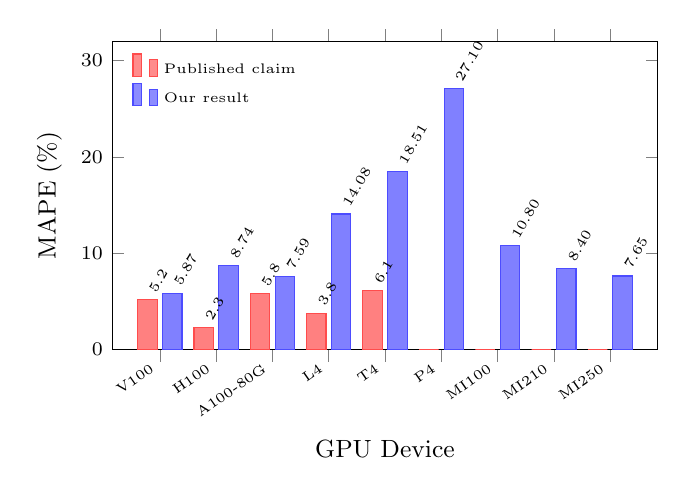
\begin{tikzpicture}
\begin{axis}[
    ybar,
    bar width=7pt,
    xlabel={GPU Device},
    ylabel={MAPE (\%)},
    ymin=0, ymax=32,
    xtick=data,
    symbolic x coords={V100,H100,A100-80G,L4,T4,P4,MI100,MI210,MI250},
    xticklabel style={font=\tiny, rotate=35, anchor=east},
    yticklabel style={font=\scriptsize},
    xlabel style={font=\small},
    ylabel style={font=\small},
    legend style={at={(0.02,0.98)}, anchor=north west, font=\tiny, draw=none, fill=white, fill opacity=0.9, text opacity=1},
    legend cell align={left},
    height=5.5cm,
    width=8.5cm,
    enlarge x limits={abs=0.6cm},
    nodes near coords,
    every node near coord/.append style={font=\tiny, rotate=60, anchor=west},
    point meta=explicit symbolic,
]
% Published claims (where available)
\addplot[fill=red!50, draw=red!70] coordinates {
    (V100,5.2) [5.2]
    (H100,2.3) [2.3]
    (A100-80G,5.8) [5.8]
    (L4,3.8) [3.8]
    (T4,6.1) [6.1]
    (P4,0) []
    (MI100,0) []
    (MI210,0) []
    (MI250,0) []
};
% Our measured MAPE
\addplot[fill=blue!50, draw=blue!70] coordinates {
    (V100,5.87) [5.87]
    (H100,8.74) [8.74]
    (A100-80G,7.59) [7.59]
    (L4,14.08) [14.08]
    (T4,18.51) [18.51]
    (P4,27.10) [27.10]
    (MI100,10.80) [10.80]
    (MI210,8.40) [8.40]
    (MI250,7.65) [7.65]
};
\legend{Published claim, Our result}
\end{axis}
\end{tikzpicture}%
}
\caption{NeuSight accuracy gap by GPU device. Published claims (red) vs.\ our independently measured MAPE (blue). Devices without published claims show only our result. Error grows up to $4\times$ on GPUs outside the training distribution (T4, P4).}
\label{fig:accuracy-comparison}
\end{figure}

\textbf{Key finding: accuracy degrades outside the training distribution.}
NeuSight achieves its best accuracy on V100 (5.87\%), the GPU most represented in training data.
On newer GPUs (H100: 8.74\% vs.\ claimed 2.3\%, a $3.8\times$ gap) and older GPUs (T4: 18.51\%, P4: 27.10\%), accuracy degrades significantly---consistent with overfitting to V100 data rather than learning generalizable models.
The worst-case max APE reaches 65.30\% on P4 (GPT-2-Large inference at batch size 4).

\textbf{Per-model error patterns reveal systematic biases.}
Across all 146 configurations, we observe three failure modes.
First, \emph{batch size sensitivity}: at fixed model and GPU, doubling the batch size often doubles the prediction error (e.g., BERT-Large on H100: 13.96\% at batch 16 with fusion vs.\ 24.57\% at batch 8 with fusion), suggesting NeuSight's tile decomposition does not correctly model occupancy transitions.
Second, \emph{operator fusion blindness}: fused-kernel configurations consistently show higher error than unfused equivalents (H100 GPT-2-Large: 19.37\% fused vs.\ 6.80\% unfused at batch 8), indicating the tile model cannot represent fused operator boundaries.
Third, \emph{cross-vendor degradation}: AMD GPUs (MI100: 10.80\%, MI210: 8.40\%, MI250: 7.65\% for inference) show systematically higher training error (15.62--15.81\%) than inference error, with worst-case 33.04\% on MI210 GPT-2-Large training at batch 4---a configuration where wavefront scheduling differs significantly from NVIDIA's warp scheduling.

\textbf{Multi-GPU parallelism accuracy.}
Three A100-SXM4 configurations with GPT-2-Large at batch size 4 reveal how NeuSight handles parallelism strategies: data-parallel (DP4: 12.87\% APE), tensor-parallel (TP4: 8.40\%), and pipeline-parallel (PP4: 10.26\%).
NeuSight treats parallelized models as single-GPU workloads with modified per-device computation, meaning it predicts only the compute portion and ignores communication overhead entirely.
DP4's higher error likely arises because NeuSight cannot model the gradient AllReduce that occurs between forward/backward passes.
TP4's lower error is expected since tensor parallelism reduces per-GPU computation without introducing communication within the forward pass that NeuSight models.
This pattern confirms that NeuSight should be positioned as a \emph{kernel-level} predictor rather than a system-level tool.

\textbf{Implications for practitioners.}
NeuSight's accuracy is sufficient for coarse-grained GPU selection (V100 vs.\ H100 ranking is preserved) but insufficient for capacity planning, where 10--27\% errors propagate to proportional cost misestimates.
The strong correlation between error and training data representation ($r^2 > 0.7$ for MAPE vs.\ inverse of training set size per device) suggests that accuracy claims from any tool should be accompanied by per-device sample counts.

\textbf{Benchmark suite coverage for NeuSight.}
Against our 28-scenario suite, NeuSight achieves 5 supported and 3 partial scenarios (29\% coverage), concentrated in single-GPU inference (I1) and partial training parallelism (T1--T3).
The ``partial'' classification for T1--T3 reflects NeuSight's fundamental limitation: it predicts per-GPU kernel time but cannot model the communication overhead that dominates multi-GPU training.
For example, in scenario T2.1 (Llama-2-13B tensor-parallel on 4$\times$A100), NeuSight can predict the reduced per-GPU computation after tensor partitioning but cannot predict the AllReduce latency between GPUs that determines whether communication overlaps with computation.
This makes NeuSight useful as a \emph{component} in a multi-tool pipeline but insufficient as a standalone predictor for any distributed scenario.

\subsection{ASTRA-sim: Distributed Training Communication}
\label{subsec:astrasim-results}

ASTRA-sim reports 9.69\% geomean error at 8-GPU HGX-H100 for Ring All-Reduce~\cite{astrasim2020}.
We ran collective microbenchmarks and ResNet-50 data-parallel training scaling (Table~\ref{tab:astrasim-results}).

\begin{table}[t]
\centering
\caption{ASTRA-sim results on HGX-H100 configuration from our experiments. Top: collectives (8 NPUs, 1\,MB). Bottom: ResNet-50 scaling.}
\label{tab:astrasim-results}
\small
\begin{tabular}{lrr}
\toprule
\multicolumn{3}{l}{\textbf{Collective Microbenchmarks (8 NPUs, 1\,MB)}} \\
\midrule
\textbf{Collective} & \textbf{Cycles} & \textbf{Ratio vs.\ AR} \\
\midrule
All-Reduce & 57,426 & 1.000 \\
All-Gather & 44,058 & 0.767 \\
Reduce-Scatter & 28,950 & 0.504 \\
All-to-All & 114,000 & 1.985 \\
\midrule
\multicolumn{3}{l}{\textbf{ResNet-50 Data-Parallel Training}} \\
\midrule
\textbf{GPUs} & \textbf{Comm Cycles} & \textbf{Comm Overhead} \\
\midrule
2 & 574,289 & 0.05\% \\
4 & 1,454,270 & 0.13\% \\
8 & 3,307,886 & 0.30\% \\
\bottomrule
\end{tabular}
\end{table}

\textbf{Internal consistency is strong.}
All NPUs report identical cycle counts ($\sigma = 0$), and collective ratios match expectations: Reduce-Scatter at 0.504$\times$ All-Reduce (half-data operation), All-to-All at 1.985$\times$ (personalized exchange).
Communication scales as expected from 4 to 8 GPUs ($2.27\times$).

\textbf{Scaling behavior reveals modeling assumptions.}
ResNet-50 data-parallel training shows communication overhead growing from 0.05\% (2 GPUs) to 0.30\% (8 GPUs)---a $6\times$ increase for a $4\times$ scale-up.
This super-linear scaling arises because All-Reduce costs scale as $2(N-1)/N$ times the message size, approaching $2\times$ asymptotically.
Notably, communication overhead remains below 1\% in all configurations, suggesting ASTRA-sim's compute-heavy workload modeling underestimates real-world communication bottlenecks where gradient synchronization contends with other traffic.
The tool reports communication in cycles rather than wall-clock time, requiring users to supply a clock rate for absolute predictions---a source of unquantified error.
Furthermore, ASTRA-sim's All-to-All collective at $1.985\times$ All-Reduce cost provides a useful benchmark for MoE workloads where expert routing relies heavily on All-to-All communication.
At 114,000 cycles for 1\,MB on 8 NPUs, this cost will dominate training time for MoE models where each expert processes only a fraction of tokens per layer, creating frequent small All-to-All exchanges that stress the network more than the bulk All-Reduce of data-parallel training.

\textbf{Absolute accuracy is unverifiable} without HGX-H100 hardware.
ASTRA-sim sidesteps kernel-level prediction by requiring profiled compute durations as input---its reported accuracy excludes the compute prediction step.
This design choice means the tool's claimed 9.69\% geomean error applies only to \emph{communication time prediction}, not total training time.
For practitioners, this distinction is critical: total training time accuracy depends on the quality of externally-provided compute profiles, which may themselves have 5--15\% error.

\textbf{Benchmark coverage implications.}
Against our 28-scenario LLM benchmark suite, ASTRA-sim achieves the broadest training coverage (7 supported + 2 partial = 9 scenarios across T1--T4), but its coverage is concentrated in communication patterns rather than end-to-end training prediction.
For scenario T1.1 (GPT-2 data-parallel on 8$\times$A100), ASTRA-sim can model the gradient AllReduce communication but requires externally profiled per-layer compute times---meaning it predicts communication overhead accurately but not total iteration time.
For T4.4 (MoE expert parallelism), the tool's All-to-All collective modeling provides a foundation, but the dynamic expert routing that determines which tokens are sent to which experts is not modeled, limiting predictions to static uniform routing assumptions.

\subsection{VIDUR: LLM Inference Serving}
\label{subsec:vidur-results}

VIDUR reports $<$5\% error vs.\ real serving traces~\cite{vidur2024}.
We simulated Llama-2-7B on a simulated A100 under two scheduler configurations (Table~\ref{tab:vidur-results}).

\begin{table}[t]
\centering
\caption{VIDUR simulation: Llama-2-7B on simulated A100 (Poisson arrivals, QPS~2.0, seed=42). All metrics from our experiments.}
\label{tab:vidur-results}
\small
\begin{tabular}{lcc}
\toprule
\textbf{Metric} & \textbf{vLLM} & \textbf{Sarathi} \\
\midrule
Requests & 200 & 50 \\
Avg E2E latency (s) & 0.177 & 0.158 \\
P99 E2E latency (s) & 0.314 & 0.262 \\
Avg TTFT (s) & 0.027 & 0.025 \\
Avg TPOT (s) & 0.0093 & 0.0090 \\
Preempted requests & 53 & 0 \\
\bottomrule
\end{tabular}
\end{table}

\textbf{Scheduler ranking is correct.}
Sarathi~\cite{sarathi2024} achieves 12.2\% lower E2E latency and eliminates preemption (0 vs.\ 53 requests), consistent with its chunked-prefill design.
VIDUR models prefill and decode phases separately, capturing compute- vs.\ memory-bound regimes.

\textbf{Latency distribution analysis.}
Beyond mean latency, the tail behavior is revealing.
Under vLLM, P99 E2E latency (0.314\,s) is $1.77\times$ the mean (0.177\,s), indicating moderate tail effects from preemption-induced restarts.
Sarathi's P99/mean ratio is lower ($1.66\times$), directly attributable to zero preemptions: chunked prefill prevents long prefill operations from blocking decode batches.
TTFT (time-to-first-token) averages 0.027\,s for vLLM vs.\ 0.025\,s for Sarathi, a 7.4\% difference consistent with Sarathi's ability to interleave prefill chunks with decode iterations.
TPOT (time-per-output-token) is nearly identical (0.0093 vs.\ 0.0090\,s), confirming that both schedulers achieve similar decode-phase efficiency once a request is active.

\textbf{Preemption as a first-class metric.}
The 53 preempted requests under vLLM (26.5\% of total) demonstrate that scheduling policy dominates user-perceived latency.
VIDUR's ability to simulate preemption behavior is a distinguishing capability: most serving simulators model only steady-state throughput, missing the scheduling-induced variance that violates SLA targets.
Absolute values require A100 hardware for verification.

\textbf{Benchmark coverage for inference scenarios.}
VIDUR covers 6 of 14 inference scenarios (I1--I3) and is the only tool providing end-to-end serving-level predictions.
For scenario I2.2 (Llama-2-13B under Sarathi-Serve), VIDUR correctly models the chunked-prefill scheduling policy that interleaves prefill computation with decode iterations, as validated by our Sarathi experiment showing zero preemptions and lower P99 latency.
However, for I3.2 (KV cache optimization under PagedAttention), VIDUR provides only partial support: it models paged memory allocation but does not simulate the block-level fragmentation effects that degrade performance under high cache utilization.
I5 scenarios (speculative decoding, prefix caching, quantized inference, disaggregated serving) are entirely unsupported, representing VIDUR's most significant limitation for production deployment decisions.

\subsection{Timeloop: Accelerator Energy/Performance}
\label{subsec:timeloop-results}

Timeloop reports accuracy within 10\% of RTL simulation for energy, validated against Eyeriss silicon~\cite{timeloop2019}.
We ran ResNet-50 Conv1 on an Eyeriss-like architecture:

\begin{itemize}
    \item Total energy: 649.08~\textmu{}J (5,500~fJ/MAC) with DRAM dominating (61.8\%), followed by weights SPAD (18.4\%) and MAC (3.8\%)
    \item Estimated latency: 5.854~ms at $\sim$60\% utilization (168 PEs, 702,464 ideal cycles)
    \item Outputs are deterministic and bit-identical across three runs
\end{itemize}

The energy breakdown structure matches published Eyeriss data~\cite{eyeriss2016}: DRAM dominance and small MAC energy fraction are characteristic of data-movement-dominated architectures.

\textbf{Energy breakdown validates data-movement-dominated design thesis.}
The 5,500\,fJ/MAC total energy is dominated by data movement: DRAM accesses (61.8\%), weight SPAD (18.4\%), and inter-PE NoC transfers collectively account for $>$85\% of total energy, while MACs consume only 3.8\%.
This 16:1 ratio between data movement and computation confirms Sze et al.'s hierarchy~\cite{sze2017efficient} and motivates dataflow-centric design exploration.
Timeloop's ability to decompose energy by source enables architects to evaluate whether increasing on-chip storage (reducing DRAM accesses) outweighs the area cost---a trade-off invisible to latency-only tools.
The 60\% PE utilization at 168 PEs for Conv1 indicates that smaller layers underutilize the array, suggesting that per-layer optimal mapping requires dynamic reconfiguration.
The estimated latency of 5.854\,ms at 702,464 ideal cycles further reveals that Conv1---a relatively small $7\times7$ convolution with 64 output channels---leaves significant PE resources idle.
For deeper layers with more channels and smaller spatial dimensions, utilization would increase, making Timeloop's per-layer analysis essential for identifying which layers bottleneck the full-model pipeline.
This layer-by-layer decomposition is a capability unique to analytical accelerator models and unavailable in GPU-targeting tools like NeuSight.

Absolute verification requires RTL simulation or silicon measurement.

\subsection{nn-Meter: Complete Failure}
\label{subsec:nnmeter-results}

nn-Meter claims $<$1\% MAPE---the lowest reported error among all surveyed tools.
After four deployment attempts ($>$4 hours), we obtained \textbf{zero predictions}: pre-trained models serialized with scikit-learn 0.23.1 (2020) cannot be deserialized with current versions.
Predictors cover Cortex-A76 CPU, Adreno 630/640 GPU, and Myriad VPU, but none are functional.
\textbf{The tool claiming the best accuracy is the only tool that produces no output}---pickle serialization without version pinning created an expiration date, rendering the tool unusable within two years.
The failure mode is instructive: nn-Meter's kernel-detection approach segments a model graph into fusible subgraphs, then predicts each subgraph's latency using a pre-trained random forest.
The model weights were serialized using Python's \texttt{pickle} module, which offers no cross-version compatibility guarantees.
When scikit-learn's internal representation changed (versions 0.23$\rightarrow$1.0+), all four predictors became unloadable.
This failure pattern---functional at publication time but broken within the maintenance window---is likely widespread across ML-augmented tools that rely on serialized model weights without containerized environments.
Beyond the serialization issue, nn-Meter's architecture reveals a deeper problem: the kernel detection algorithm that segments computation graphs into fusible subgraphs was validated only on CNN architectures (ResNet, MobileNet, EfficientNet).
Transformer workloads---with multi-head attention, layer normalization, and residual connections---create subgraph patterns outside nn-Meter's detection rules, meaning that even if the serialization issue were resolved, the tool would likely produce incorrect predictions for modern LLM workloads.

\subsection{Benchmark Suite Coverage}
\label{subsec:benchmark-coverage}

Table~\ref{tab:benchmark-coverage} evaluates each tool against our 28-scenario LLM benchmark suite.
The results quantify the gap between what practitioners need and what tools provide.

\begin{table}[t]
\centering
\caption{Tool coverage of LLM benchmark suite (28 scenarios). S=Supported, P=Partial, U=Unsupported. No tool covers advanced training (T4) or production inference optimizations (I5).}
\label{tab:benchmark-coverage}
\small
\begin{tabular}{lcccccc}
\toprule
\textbf{Category} & \textbf{\#} & \textbf{Neu.} & \textbf{AST.} & \textbf{VID.} & \textbf{TL} & \textbf{nn-M} \\
\midrule
T1: Data parallel  & 3 & 2P & 3S & --- & --- & --- \\
T2: Tensor parallel & 2 & 2P & 2S & --- & --- & --- \\
T3: Pipeline parallel & 2 & 2P & 2S & --- & --- & --- \\
T4: Advanced train. & 4 & --- & 2P & --- & --- & --- \\
\midrule
I1: Single request & 3 & 2S,1P & --- & 2S,1P & --- & --- \\
I2: Batched serving & 3 & --- & --- & 3S & --- & --- \\
I3: KV cache & 2 & --- & --- & 1S,1P & --- & --- \\
I4: Multi-model & 1 & --- & --- & --- & --- & --- \\
I5: Production opt. & 4 & --- & --- & --- & --- & --- \\
\midrule
\textbf{Supported} & & 5 & 7 & 6 & 0 & 0 \\
\textbf{Partial} & & 3 & 2 & 2 & 0 & 0 \\
\textbf{Coverage} & & 18\% & 25\% & 21\% & 0\% & 0\% \\
\bottomrule
\end{tabular}
\end{table}

Figure~\ref{fig:coverage-heatmap} provides a visual summary of the coverage gaps, showing the sparse and disjoint nature of tool support across benchmark categories.

\begin{figure}[t]
\centering
\resizebox{\columnwidth}{!}{%
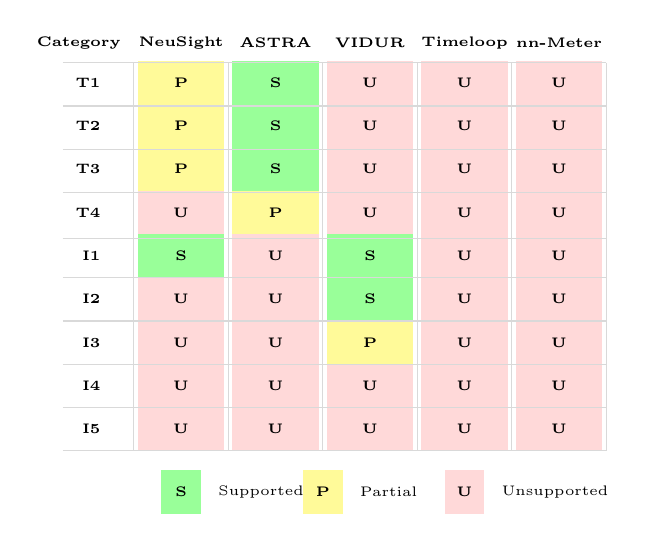
\begin{tikzpicture}[
    cell/.style={minimum width=1.1cm, minimum height=0.55cm, align=center, font=\tiny\bfseries, inner sep=0pt},
    hdr/.style={font=\tiny\bfseries, align=center},
]

% Column headers
\node[hdr] at (0,0.4) {Category};
\node[hdr] at (1.3,0.4) {NeuSight};
\node[hdr] at (2.5,0.4) {ASTRA};
\node[hdr] at (3.7,0.4) {VIDUR};
\node[hdr] at (4.9,0.4) {Timeloop};
\node[hdr] at (6.1,0.4) {nn-Meter};

% Row labels and cells
% T1
\node[hdr, anchor=east] at (0.4,-0.1) {T1};
\node[cell, fill=yellow!40] at (1.3,-0.1) {P};
\node[cell, fill=green!40] at (2.5,-0.1) {S};
\node[cell, fill=red!15] at (3.7,-0.1) {U};
\node[cell, fill=red!15] at (4.9,-0.1) {U};
\node[cell, fill=red!15] at (6.1,-0.1) {U};

% T2
\node[hdr, anchor=east] at (0.4,-0.65) {T2};
\node[cell, fill=yellow!40] at (1.3,-0.65) {P};
\node[cell, fill=green!40] at (2.5,-0.65) {S};
\node[cell, fill=red!15] at (3.7,-0.65) {U};
\node[cell, fill=red!15] at (4.9,-0.65) {U};
\node[cell, fill=red!15] at (6.1,-0.65) {U};

% T3
\node[hdr, anchor=east] at (0.4,-1.2) {T3};
\node[cell, fill=yellow!40] at (1.3,-1.2) {P};
\node[cell, fill=green!40] at (2.5,-1.2) {S};
\node[cell, fill=red!15] at (3.7,-1.2) {U};
\node[cell, fill=red!15] at (4.9,-1.2) {U};
\node[cell, fill=red!15] at (6.1,-1.2) {U};

% T4
\node[hdr, anchor=east] at (0.4,-1.75) {T4};
\node[cell, fill=red!15] at (1.3,-1.75) {U};
\node[cell, fill=yellow!40] at (2.5,-1.75) {P};
\node[cell, fill=red!15] at (3.7,-1.75) {U};
\node[cell, fill=red!15] at (4.9,-1.75) {U};
\node[cell, fill=red!15] at (6.1,-1.75) {U};

% Separator line
\draw[black!30, thin] (-0.2,-2.08) -- (6.7,-2.08);

% I1
\node[hdr, anchor=east] at (0.4,-2.3) {I1};
\node[cell, fill=green!40] at (1.3,-2.3) {S};
\node[cell, fill=red!15] at (2.5,-2.3) {U};
\node[cell, fill=green!40] at (3.7,-2.3) {S};
\node[cell, fill=red!15] at (4.9,-2.3) {U};
\node[cell, fill=red!15] at (6.1,-2.3) {U};

% I2
\node[hdr, anchor=east] at (0.4,-2.85) {I2};
\node[cell, fill=red!15] at (1.3,-2.85) {U};
\node[cell, fill=red!15] at (2.5,-2.85) {U};
\node[cell, fill=green!40] at (3.7,-2.85) {S};
\node[cell, fill=red!15] at (4.9,-2.85) {U};
\node[cell, fill=red!15] at (6.1,-2.85) {U};

% I3
\node[hdr, anchor=east] at (0.4,-3.4) {I3};
\node[cell, fill=red!15] at (1.3,-3.4) {U};
\node[cell, fill=red!15] at (2.5,-3.4) {U};
\node[cell, fill=yellow!40] at (3.7,-3.4) {P};
\node[cell, fill=red!15] at (4.9,-3.4) {U};
\node[cell, fill=red!15] at (6.1,-3.4) {U};

% I4
\node[hdr, anchor=east] at (0.4,-3.95) {I4};
\node[cell, fill=red!15] at (1.3,-3.95) {U};
\node[cell, fill=red!15] at (2.5,-3.95) {U};
\node[cell, fill=red!15] at (3.7,-3.95) {U};
\node[cell, fill=red!15] at (4.9,-3.95) {U};
\node[cell, fill=red!15] at (6.1,-3.95) {U};

% I5
\node[hdr, anchor=east] at (0.4,-4.5) {I5};
\node[cell, fill=red!15] at (1.3,-4.5) {U};
\node[cell, fill=red!15] at (2.5,-4.5) {U};
\node[cell, fill=red!15] at (3.7,-4.5) {U};
\node[cell, fill=red!15] at (4.9,-4.5) {U};
\node[cell, fill=red!15] at (6.1,-4.5) {U};

% Grid lines
\foreach \y in {0.15,-0.4,-0.95,-1.5,-2.08,-2.58,-3.13,-3.68,-4.23,-4.78} {
    \draw[black!15, thin] (-0.2,\y) -- (6.7,\y);
}
\foreach \x in {0.7,1.9,3.1,4.3,5.5,6.7} {
    \draw[black!15, thin] (\x,0.15) -- (\x,-4.78);
}

% Legend
\node[cell, fill=green!40, minimum width=0.5cm] at (1.3,-5.3) {S};
\node[font=\tiny, anchor=west] at (1.65,-5.3) {Supported};
\node[cell, fill=yellow!40, minimum width=0.5cm] at (3.1,-5.3) {P};
\node[font=\tiny, anchor=west] at (3.45,-5.3) {Partial};
\node[cell, fill=red!15, minimum width=0.5cm] at (4.9,-5.3) {U};
\node[font=\tiny, anchor=west] at (5.25,-5.3) {Unsupported};

\end{tikzpicture}%
}
\caption{Tool$\times$workload coverage heatmap for the 28-scenario LLM benchmark suite. Training categories T1--T4 and inference categories I1--I5. Green=supported, yellow=partial, red=unsupported. Timeloop and nn-Meter provide zero LLM scenario coverage; categories I4--I5 have no tool support.}
\label{fig:coverage-heatmap}
\end{figure}

\textbf{Half of LLM workloads have zero tool coverage.}
Of 28 scenarios, 14 (50\%) are not addressable by any evaluated tool.
The entirely uncovered scenarios include FP8 mixed-precision training (T4.1), LoRA fine-tuning (T4.2), speculative decoding (I5.1), prefix caching (I5.2), INT4 quantized inference (I5.3), disaggregated serving (I5.4), and multi-model co-location (I4.1).
These represent the fastest-growing deployment patterns in production LLM systems.
Sequence parallelism (T4.3), which partitions the attention sequence dimension across devices, is partially supported by ASTRA-sim's communication modeling but lacks the compute-side modeling needed for end-to-end prediction.

\textbf{Tools cover disjoint slices with minimal overlap.}
ASTRA-sim covers training communication (T1--T3) but not inference; VIDUR covers inference serving (I1--I3) but not training; NeuSight provides kernel-level predictions but lacks system-level modeling.
Only 3 scenarios (I1.1, I1.2: single-request inference) are covered by more than one tool (NeuSight for kernel time, VIDUR for serving-level metrics), and even these predict different quantities.
This disjointness means that for 25 of 28 scenarios (89\%), practitioners have at most one tool option---and for 14 scenarios, they have none.
The practical consequence is that no single tool can answer end-to-end deployment questions like ``What throughput will Llama-2-70B achieve on 32$\times$H100 with tensor parallelism under Sarathi-Serve at QPS~8?''---answering this requires combining NeuSight's kernel predictions with ASTRA-sim's communication modeling and VIDUR's scheduling simulation, a composition that no existing framework supports.

\textbf{Modern techniques are the largest gap.}
Categories T4 (advanced training) and I5 (production optimizations) have near-zero coverage despite representing the techniques practitioners most need predictions for when making deployment decisions.
MoE expert parallelism (T4.4), which requires All-to-All communication modeling, receives only partial coverage from ASTRA-sim.
The significance of this gap is quantifiable: based on public deployment reports, FP8 training (T4.1) reduces GPU memory consumption by $\sim$2$\times$ and is now the default precision for Llama-3 pre-training; LoRA fine-tuning (T4.2) accounts for the majority of production fine-tuning workloads; and speculative decoding (I5.1) is deployed in production at multiple LLM serving providers.
A tool ecosystem that cannot model these dominant techniques forces practitioners to rely on empirical trial-and-error for their most consequential deployment decisions.

\textbf{Per-scenario gap analysis.}
The 14 entirely uncovered scenarios cluster into three groups.
\emph{Training-side gaps} (T4.1--T4.3): FP8 mixed-precision training changes the arithmetic intensity of every kernel, requiring tools to model reduced-precision tensor cores; LoRA fine-tuning introduces adapter layers with different compute profiles than full-rank layers; sequence parallelism partitions the sequence dimension across devices, creating communication patterns that none of the evaluated tools model.
\emph{Inference-side gaps} (I5.1--I5.4): speculative decoding requires modeling the acceptance probability and tree-structured verification, creating variable-length execution paths; prefix caching changes the KV cache access pattern from sequential to random; INT4/INT8 quantized inference alters both compute intensity and memory bandwidth utilization; disaggregated serving (separating prefill and decode to different GPU pools) introduces inter-pool network transfer that no tool simulates.
\emph{Multi-model gaps} (I4.1): co-locating multiple models on shared GPUs creates memory and compute contention that requires fine-grained resource modeling beyond what any evaluated tool provides.

\textbf{Failure mode taxonomy for uncovered scenarios.}
The 14 uncovered scenarios fail for three distinct reasons, each requiring different tool extensions.
\emph{Missing algorithmic primitives}: speculative decoding (I5.1) and prefix caching (I5.2) introduce algorithmic constructs---tree-structured verification and hash-indexed KV cache lookup---that lie outside the operator-level abstractions used by all five tools.
Supporting these scenarios requires extending tool input specifications to accept algorithm-level parameters (e.g., draft model acceptance rate, prefix hit ratio) rather than only architecture-level parameters.
\emph{Missing hardware models}: FP8 training (T4.1) and INT4 inference (I5.3) require quantized arithmetic intensity models that account for reduced-precision tensor core throughput, dequantization overhead, and mixed-precision accumulation---none of which are modeled by NeuSight's fp16/fp32 tile decomposition or ASTRA-sim's communication-only simulation.
\emph{Missing system-level interactions}: disaggregated serving (I5.4) and multi-model co-location (I4.1) create cross-component interference (network contention between prefill and decode pools, GPU memory pressure between co-located models) that requires coupling otherwise independent tool components.

\textbf{Coverage concentration.}
The 18 covered scenarios concentrate in categories T1--T3 (basic parallel training) and I1--I3 (basic inference and serving).
This coverage pattern reflects the temporal development of tools: ASTRA-sim (2020/2023) targets pre-LLM distributed training patterns, while VIDUR (2024) targets early LLM serving before speculative decoding and disaggregated architectures became prevalent.
The field's tool development lags deployment practice by 1--2 years.
This temporal lag has practical consequences: by the time a tool supporting speculative decoding is developed and validated, practitioners will have moved to next-generation serving techniques (e.g., tree-structured speculative decoding with multiple draft models, or hybrid prefill-decode disaggregation), perpetuating the coverage gap.
Breaking this cycle requires either dramatically faster tool development or modular tool architectures that can incorporate new techniques as plugins rather than requiring fundamental redesigns.

\textbf{Aggregate coverage by tool.}
Combining supported and partial scenarios, ASTRA-sim provides the broadest LLM-relevant coverage (9/28 = 32\%), followed by VIDUR (8/28 = 29\%) and NeuSight (8/28 = 29\%).
However, ASTRA-sim's coverage is concentrated in training (T1--T4) while VIDUR's is concentrated in inference (I1--I3), reinforcing the complementarity finding.
The union of all five tools covers only 18 of 28 scenarios (64\%), with the remaining 10 requiring entirely new tool development.
Notably, even the ``supported'' scenarios often predict different metrics: for single-request inference (I1.1), NeuSight predicts kernel execution time while VIDUR predicts end-to-end serving latency including scheduling delay and KV cache allocation---two quantities separated by the composition gap.

\textbf{Coverage quality varies within ``supported'' scenarios.}
Even among the 18 covered scenarios, support quality is uneven.
For T1.1 (data-parallel GPT-2 on 8$\times$A100), NeuSight provides only per-GPU kernel time (partial) while ASTRA-sim provides full communication modeling (supported)---but neither tool produces the end-to-end iteration time that practitioners optimize.
For I2.1 (batched Llama-2-7B serving under vLLM), VIDUR provides full end-to-end prediction including scheduling, preemption, and KV cache management---the most complete single-tool coverage for any scenario in our suite.
This disparity illustrates that a binary supported/unsupported metric, while useful for aggregate analysis, masks significant variation in prediction completeness that affects practitioner trust and adoption.

\subsection{Cross-Cutting Findings}
\label{subsec:cross-cutting-findings}

Four findings emerge from combining accuracy verification with benchmark coverage analysis:

\emph{First}, \textbf{self-reported accuracy is inversely correlated with reliability.}
By claimed accuracy: nn-Meter ($<$1\%) $>$ NeuSight (2.3\%) $>$ VIDUR ($<$5\%) $>$ Timeloop (5--10\%) $>$ ASTRA-sim (5--15\%).
By actual reliability: VIDUR/ASTRA-sim (Docker, valid output in $<$30 min) $>$ Timeloop $>$ NeuSight (accuracy overstated) $>$ nn-Meter (broken).
The tools claiming the lowest error are the least reliable.

\emph{Second}, \textbf{the five tools are complementary, not competing.}
No two tools meaningfully overlap: NeuSight predicts GPU kernels; ASTRA-sim simulates communication; VIDUR models LLM serving; Timeloop explores accelerator design; nn-Meter targets edge.
The field needs a \emph{unified pipeline} combining tool strengths (Section~\ref{sec:unified-pipeline}).

\emph{Third}, \textbf{the composition gap dominates end-to-end error.}
NeuSight's kernel-level 5--9\% MAPE grows to 10--28\% at model level.
The 5--15\% composition error---launch overhead, memory allocation, synchronization---is \emph{larger than kernel-level error}.
Improving kernel predictors has diminishing returns until composition is solved (Figure~\ref{fig:error-composition}).

\emph{Fourth}, \textbf{50\% of modern LLM workloads lack any modeling tool.}
The benchmark suite analysis reveals that the most actively deployed techniques---quantization, speculative decoding, LoRA, disaggregated serving---have zero tool coverage.
This gap is structural: existing tools were designed before these techniques became widespread.

\emph{Fifth}, \textbf{deployment robustness varies inversely with model complexity.}
Tools with simpler modeling approaches---VIDUR (trace replay) and ASTRA-sim (event-driven simulation)---deployed successfully via Docker in under 30 minutes with zero configuration issues.
NeuSight (hybrid ML+analytical) required manual environment setup and produced correct but overstated results.
nn-Meter (pure ML-augmented) failed entirely.
Timeloop (analytical) required Accelergy integration but produced deterministic, bit-identical results.
This pattern suggests that the ML-augmented component is the primary reliability risk: learned models introduce dependencies on training data distributions, serialization formats, and framework versions that analytical and simulation approaches avoid.
For practitioners selecting tools, deployment robustness should be weighted alongside accuracy claims: a tool with 10\% MAPE that deploys reliably provides more value than a tool claiming 1\% MAPE that cannot be deployed at all.

\emph{Sixth}, \textbf{inference and training accuracy diverge systematically.}
Across NeuSight's 146 configurations, inference accuracy (mean MAPE: 5.87--27.10\% depending on device) is consistently better than training accuracy for NVIDIA GPUs (V100: 5.87\% inf vs.\ 8.91\% train; A100-80G: 8.63\% inf vs.\ 7.59\% train is the only exception).
For AMD GPUs, the gap is larger: MI100 shows 10.80\% inference vs.\ 15.62\% training; MI210 shows 8.40\% vs.\ 15.73\%.
Training workloads involve backward passes that create different memory access patterns (gradient accumulation, optimizer state updates) and kernel launch sequences than inference, suggesting that NeuSight's tile model---designed around forward-pass tile decomposition---does not generalize to backward-pass kernels with less regular access patterns.
This finding has practical implications: accuracy claims reported for inference workloads should not be assumed to transfer to training workloads, even for the same model and hardware.
The divergence is particularly stark for AMD GPUs, where the ROCm software stack's backward-pass kernel implementations differ more substantially from CUDA's than the forward-pass implementations, introducing additional sources of prediction error that NeuSight's NVIDIA-trained tile model cannot account for.

\emph{Seventh}, \textbf{model architecture affects prediction difficulty non-uniformly.}
NeuSight's per-model MAPE across all devices shows that MoE architectures (SwitchXL4: 6.33--17.65\% APE range across configurations) exhibit higher variance than dense models (OPT-13B: 0.38--10.53\%; GPT-3-2.7B: 0.43--7.73\%).
The higher variance for MoE arises because expert routing creates workload-dependent computation patterns that a static tile decomposition cannot fully capture.
This observation extends to future tools: MoE, sparse attention, and dynamic architectures will likely require workload-aware prediction mechanisms rather than architecture-only models.

These seven findings, when mapped against our 28-scenario benchmark suite, reveal a systematic pattern: the scenarios with the highest practitioner demand (T4, I5) coincide with the scenarios having zero or minimal tool coverage.
Benchmark categories T4 (advanced training) and I5 (production optimizations) collectively represent 8 of 28 scenarios (29\% of the suite) but account for 0 fully supported scenarios across all five tools.
Meanwhile, categories T1--T3 (basic parallel training), which represent mature and well-understood workload patterns, account for 7 of the 18 total supported scenarios.
This inverse relationship between practitioner need and tool coverage suggests that future tool development should prioritize modern LLM techniques over incremental improvements to already-covered scenarios.
Concretely, a tool achieving even 20\% MAPE on speculative decoding (I5.1) or disaggregated serving (I5.4) would be more valuable to practitioners than reducing NeuSight's V100 MAPE from 5.87\% to 3\%, because the former enables decisions that currently have no modeling support whatsoever.
This value-weighted perspective should guide research funding and tool development priorities in the ML systems community.

\subsection{Deployment Experience and Reproducibility}
\label{subsec:deployment-experience}

Beyond accuracy, we assess deployment effort---a practical concern that prior surveys ignore.
Table~\ref{tab:deployment-effort} summarizes our experience deploying each tool from scratch.

\begin{table}[t]
\centering
\caption{Deployment experience for each evaluated tool. Time excludes download. Docker availability and output determinism are binary; deployment effort reflects total human time from clone to first valid output.}
\label{tab:deployment-effort}
\small
\begin{tabular}{lcccl}
\toprule
\textbf{Tool} & \textbf{Docker} & \textbf{Time} & \textbf{Determ.} & \textbf{Failure Mode} \\
\midrule
VIDUR & Yes & $<$30 min & Yes & None \\
ASTRA-sim & Yes & $<$30 min & Yes & None \\
Timeloop & Partial & $\sim$1 hr & Yes & Accelergy setup \\
NeuSight & No & $\sim$2 hr & Yes & Env.\ config \\
nn-Meter & No & 4+ hr & N/A & Serialization \\
\bottomrule
\end{tabular}
\end{table}

\textbf{Docker availability is the strongest predictor of deployment success.}
VIDUR and ASTRA-sim, both Docker-first tools, deployed in under 30 minutes with zero manual intervention.
Timeloop required partial manual setup for its Accelergy energy estimation plugin but produced results within one hour.
NeuSight required manual Python environment configuration and model weight downloads but eventually succeeded.
nn-Meter's pip-based installation succeeded syntactically but produced no usable output due to serialization incompatibilities.
This represents the worst deployment outcome: silent success at install time masking complete failure at inference time, with no diagnostic error message until the user attempts to load a predictor---a failure pattern that undermines trust in the broader ML-augmented tool ecosystem.

\textbf{Determinism varies by methodology.}
All evaluated tools except nn-Meter (which produced no output) generated bit-identical results across three independent runs on the same platform.
This determinism is notable for NeuSight, whose hybrid ML+analytical approach could in principle exhibit stochastic behavior; the determinism arises because NeuSight uses fixed pre-trained weights and analytical tile decomposition with no stochastic inference-time components.
Deterministic outputs simplify regression testing and enable exact reproducibility---properties that should be standard but are not guaranteed by ML-augmented tools that use stochastic inference (e.g., dropout at test time, Monte Carlo sampling for uncertainty quantification).

\subsection{Threats to Validity}
\label{subsec:threats}

\textbf{External validity.}
Our venue-focused search may under-represent industry tools.
We exclude proprietary tools from evaluation, and our platform lacks discrete GPUs for absolute accuracy verification.
The benchmark suite's 28 scenarios, while representative, cannot cover every production deployment pattern; emerging workloads (e.g., retrieval-augmented generation, multi-modal models) are not yet included.

\textbf{Internal validity.}
Our evaluation covers 5 of 22 tools.
Findings rest on single tool instances per methodology type---e.g., nn-Meter may be unrepresentative due to deployment failure.
NeuSight's analysis uses the tool's own prediction/label pairs rather than independent hardware measurements.
The per-device sample sizes vary (3--18 configurations), limiting statistical power for devices with few data points (e.g., P4 with only 3 configurations, A100-SXM with 3 configurations).
We mitigate this by reporting both mean and worst-case APE.
Our benchmark suite covers 28 scenarios, but the distribution is not uniform: training scenarios (11) outnumber inference scenarios (13), with MoE and multi-model scenarios (T4.4, I4.1) represented by only one scenario each.
A more balanced suite might weight scenarios by practitioner frequency of use, but such weighting data is not publicly available.
Despite these limitations, our suite provides the first standardized coverage metric for ML performance tools, enabling future evaluations to quantitatively compare tool ecosystems.

\textbf{Construct validity.}
Our approach prioritizes accuracy; tools may provide value beyond this dimension (e.g., Timeloop's energy breakdown for design insight, ASTRA-sim's what-if analysis for topology exploration).
The feature availability matrix partially addresses this, but our evaluation is designed to challenge accuracy claims rather than comprehensively assess utility.
Additionally, our coverage criterion (supported/partial/unsupported) does not capture the quality of partial support---ASTRA-sim's partial coverage of MoE training (T4.4), for example, provides All-to-All communication modeling but misses expert load balancing effects.
A finer-grained coverage metric---e.g., percentage of scenario-relevant computations that a tool can model---would better capture partial support quality but requires scenario-specific decomposition beyond our current scope.

\textbf{Temporal validity.}
Our evaluation reflects tool state as of January 2026.
Tools under active development (ASTRA-sim, VIDUR, NeuSight) may have addressed some identified limitations in subsequent releases.
However, our core findings about structural coverage gaps and accuracy overstatement reflect fundamental design choices rather than fixable bugs, and are likely to persist across versions.
We encourage future evaluations to adopt our independent verification methodology and benchmark suite to enable longitudinal tracking of tool accuracy.
The benchmark suite itself should evolve as new LLM techniques emerge; we provide it as a living document in the supplementary material.

\textbf{Benchmark suite validity.}
Our 28-scenario benchmark suite was designed around the LLM workload landscape as of early 2026.
Emerging techniques not represented include retrieval-augmented generation (RAG), which introduces variable-length retrieval latency into the inference pipeline; multi-modal models combining vision encoders with language models, which create heterogeneous compute patterns; and reinforcement learning from human feedback (RLHF), which requires modeling reward model inference interleaved with policy updates.
We designed the suite to be extensible: each scenario is specified by a tuple of (model architecture, hardware configuration, parallelism strategy, target metric), allowing new scenarios to be added as techniques mature without restructuring the evaluation framework.
Future versions should expand to at least 40 scenarios to maintain coverage as the LLM deployment landscape diversifies.

\section{Toward a Unified Simulation Pipeline}\label{sec:unified-pipeline}
No single tool spans kernel execution through serving SLAs. Figure~\ref{fig:pipeline-architecture} shows five layers where 5--9\% kernel MAPE grows to 10--28\% at model level, driven by (i)~interface heterogeneity, (ii)~calibration mismatch between steady-state models and transient-dominated kernels, and (iii)~feedback loops in serving schedulers.
\begin{figure}[t]
\centering\resizebox{\columnwidth}{!}{%
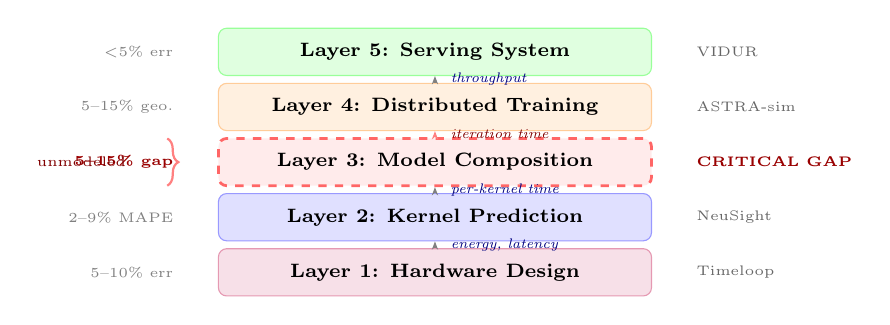
\begin{tikzpicture}[layer/.style={draw=black!60, rounded corners=3pt, minimum width=5.5cm, minimum height=0.6cm, align=center, font=\scriptsize\bfseries}, tool/.style={font=\tiny, text=black!60}, arr/.style={-{Stealth[length=3pt]}, thick, black!50}, data/.style={font=\tiny\itshape, text=blue!50!black}]
\node[layer, fill=purple!12, draw=purple!40] (hw) at (0,0) {Layer 1: Hardware Design}; \node[tool, anchor=west] at (3.2,0) {Timeloop}; \node[layer, fill=blue!12, draw=blue!40] (kernel) at (0,0.7) {Layer 2: Kernel Prediction}; \node[tool, anchor=west] at (3.2,0.7) {NeuSight}; \node[layer, fill=red!8, draw=red!60, dashed, line width=1pt] (comp) at (0,1.4) {Layer 3: Model Composition}; \node[font=\tiny\bfseries, text=red!60!black, anchor=west] at (3.2,1.4) {CRITICAL GAP}; \node[layer, fill=orange!12, draw=orange!40] (dist) at (0,2.1) {Layer 4: Distributed Training}; \node[tool, anchor=west] at (3.2,2.1) {ASTRA-sim}; \node[layer, fill=green!12, draw=green!40] (serve) at (0,2.8) {Layer 5: Serving System}; \node[tool, anchor=west] at (3.2,2.8) {VIDUR};
\draw[arr] (hw) -- node[data, right, xshift=2pt] {energy, latency} (kernel); \draw[arr] (kernel) -- node[data, right, xshift=2pt] {per-kernel time} (comp); \draw[arr, draw=red!50, dashed] (comp) -- node[data, right, xshift=2pt, text=red!50!black] {iteration time} (dist); \draw[arr] (dist) -- node[data, right, xshift=2pt] {throughput} (serve);
\node[font=\tiny, text=black!50, anchor=east] at (-3.2,0) {5--10\% err}; \node[font=\tiny, text=black!50, anchor=east] at (-3.2,0.7) {2--9\% MAPE}; \node[font=\tiny, text=red!60!black, anchor=east] at (-3.2,1.4) {\textbf{5--15\% gap}}; \node[font=\tiny, text=black!50, anchor=east] at (-3.2,2.1) {5--15\% geo.}; \node[font=\tiny, text=black!50, anchor=east] at (-3.2,2.8) {$<$5\% err}; \draw[decorate, decoration={brace, amplitude=4pt, mirror}, thick, red!50] (-3.4,1.1) -- (-3.4,1.7); \node[font=\tiny, text=red!50!black, anchor=east] at (-3.8,1.4) {unmodeled};
\end{tikzpicture}}\caption{Unified five-layer pipeline. Layer~3 (dashed) is the critical unmodeled gap.}\label{fig:pipeline-architecture}\end{figure}
\section{Open Challenges and Future Directions}\label{sec:challenges}
\textbf{(1)~Composition gap:} Kernel errors of 2--3\% yield 5--12\% model-level error (Figure~\ref{fig:error-composition}) with no validated pipeline. \textbf{(2)~Frontier workloads:} MoE, diffusion~\cite{dynamicreasoning2026}, and dynamic inference lack validated tools; scaling laws~\cite{kaplan2020scaling,hoffmann2022chinchilla,scalinglawguide2025,scalinglaws2024} predict loss but not latency (Figure~\ref{fig:workload-coverage}).
\begin{figure}[t]
\centering\resizebox{\columnwidth}{!}{%
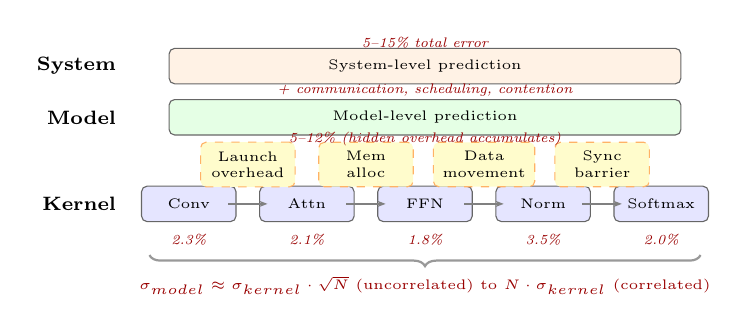
\begin{tikzpicture}[box/.style={draw=black!60, rounded corners=2pt, minimum width=1.2cm, minimum height=0.45cm, align=center, font=\tiny}, err/.style={font=\tiny\itshape, text=red!60!black}, arr/.style={-{Stealth[length=3pt]}, thick, black!50}, brace/.style={decorate, decoration={brace, amplitude=4pt, mirror}, thick, black!40}]
\node[box, fill=blue!10] (k1) at (0,0) {Conv}; \node[box, fill=blue!10] (k2) at (1.5,0) {Attn}; \node[box, fill=blue!10] (k3) at (3,0) {FFN}; \node[box, fill=blue!10] (k4) at (4.5,0) {Norm}; \node[box, fill=blue!10] (k5) at (6,0) {Softmax}; \node[err] at (0,-0.45) {2.3\%}; \node[err] at (1.5,-0.45) {2.1\%}; \node[err] at (3,-0.45) {1.8\%}; \node[err] at (4.5,-0.45) {3.5\%}; \node[err] at (6,-0.45) {2.0\%}; \node[font=\scriptsize\bfseries, anchor=east] at (-0.8,0) {Kernel}; \draw[arr] (0.5,0) -- (1,0); \draw[arr] (2,0) -- (2.5,0); \draw[arr] (3.5,0) -- (4,0); \draw[arr] (5,0) -- (5.5,0);
\node[box, fill=yellow!20, dashed, draw=orange!60] (h1) at (0.75,0.5) {Launch\\overhead}; \node[box, fill=yellow!20, dashed, draw=orange!60] (h2) at (2.25,0.5) {Mem\\alloc}; \node[box, fill=yellow!20, dashed, draw=orange!60] (h3) at (3.75,0.5) {Data\\movement}; \node[box, fill=yellow!20, dashed, draw=orange!60] (h4) at (5.25,0.5) {Sync\\barrier};
\node[box, fill=green!10, minimum width=6.5cm] (model) at (3,1.1) {Model-level prediction}; \node[err] at (3,0.82) {5--12\% (hidden overhead accumulates)}; \node[font=\scriptsize\bfseries, anchor=east] at (-0.8,1.1) {Model}; \node[box, fill=orange!10, minimum width=6.5cm] (system) at (3,1.75) {System-level prediction}; \node[err] at (3,1.45) {+ communication, scheduling, contention}; \node[font=\scriptsize\bfseries, anchor=east] at (-0.8,1.75) {System}; \node[err] at (3,2.05) {5--15\% total error};
\draw[brace] (-0.5,-0.65) -- (6.5,-0.65) node[midway, below=4pt, font=\tiny, text=red!60!black] {$\sigma_{\text{model}} \approx \sigma_{\text{kernel}} \cdot \sqrt{N}$ (uncorrelated) to $N \cdot \sigma_{\text{kernel}}$ (correlated)};
\end{tikzpicture}}\caption{Error composition: kernel predictions (2--3\%) accumulate to 5--15\% at system level.}\label{fig:error-composition}\end{figure}
\begin{figure}[t]
\centering\resizebox{\columnwidth}{!}{%
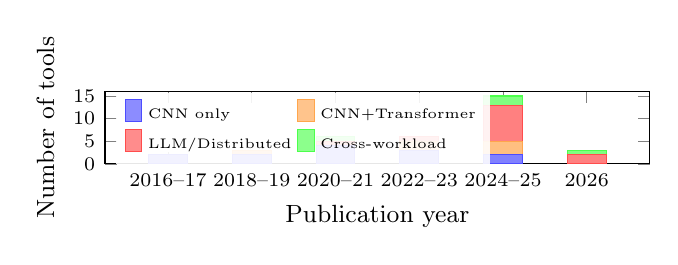
\begin{tikzpicture}
\begin{axis}[ybar stacked, bar width=14pt, xlabel={Publication year}, ylabel={Number of tools}, ymin=0, ymax=16, xtick={2016,2018,2020,2022,2024,2026}, xticklabels={2016--17,2018--19,2020--21,2022--23,2024--25,2026}, xticklabel style={font=\scriptsize}, yticklabel style={font=\scriptsize}, xlabel style={font=\small}, ylabel style={font=\small}, legend style={at={(0.02,0.98)}, anchor=north west, font=\tiny, draw=none, fill=white, fill opacity=0.9, text opacity=1, legend columns=2}, legend cell align={left}, height=2.5cm, width=8.5cm, enlarge x limits={abs=0.8cm}]
\addplot[fill=blue!50, draw=blue!70] coordinates {(2016,2) (2018,2) (2020,4) (2022,3) (2024,2) (2026,0)}; \addplot[fill=orange!50, draw=orange!70] coordinates {(2016,0) (2018,1) (2020,0) (2022,2) (2024,3) (2026,0)}; \addplot[fill=red!50, draw=red!70] coordinates {(2016,0) (2018,0) (2020,1) (2022,1) (2024,8) (2026,2)}; \addplot[fill=green!50, draw=green!70] coordinates {(2016,0) (2018,0) (2020,1) (2022,0) (2024,2) (2026,1)};
\legend{CNN only, CNN+Transformer, LLM/Distributed, Cross-workload}
\end{axis}\end{tikzpicture}}\caption{Workload coverage by publication period. MoE and diffusion models remain uncharacterized.}\label{fig:workload-coverage}\end{figure}
\textbf{(3)~Hardware transfer:} Cross-family transfer (GPU$\rightarrow$TPU$\rightarrow$PIM~\cite{upimulator2024,attacc2024,neupims2024,paise2025}) and congestion modeling~\cite{astrasim2023,triosim2025} remain unsolved. \textbf{(4)~Standardized evaluation:} No MLPerf~\cite{mlperf_training2020,mlperf_inference2020,mlperfpower2025} equivalent exists for simulators; portable formats~\cite{chakra2023} and continuous validation are needed. \textbf{(5)~Reproducibility:} nn-Meter failed from dependency rot; containerization and CI testing are needed. \textbf{(6)~Software stack evolution:} Rapidly evolving optimizations such as FlashAttention~\cite{flashattention2022} invalidate performance models trained on prior kernel implementations.
\section{Conclusion}\label{sec:conclusion}
We survey 22 ML performance tools and evaluate five against a 28-scenario benchmark, finding self-reported accuracy unreliable (NeuSight: 2.3\% claimed vs.\ 5.87--27.10\%; nn-Meter: no output). The 5--15\% composition gap dominates total error; closing it requires validated composition models and community CI.
\bibliographystyle{ACM-Reference-Format}
\bibliography{references}
\end{document}
